\documentclass[utf8]{ctexart}

\usepackage[a4paper,left=1.25in,right=1.25in,top=1in,bottom=1in]{geometry}
\usepackage{listings}
\usepackage{graphicx}
\usepackage{caption}
\usepackage{subfigure}
\usepackage{booktabs}
\usepackage{amsmath}
\usepackage{amsthm}
\usepackage{amsfonts}
\usepackage{float}
\usepackage{indentfirst}
\usepackage{tikz}
\usetikzlibrary{shapes,arrows}
\usetikzlibrary{shapes.geometric, arrows}
\usepackage{algorithm}
\usepackage{algorithmic}
\usepackage{newclude}
\usepackage[perpage]{footmisc}

\graphicspath{ {images/} }
\raggedbottom	% 令页面在垂直方向向顶部对齐
\renewcommand\qedsymbol{QED}
\newcommand{\sign}[1]{\mathrm{sgn}(#1)}
\everymath{\displaystyle}   % 行内公式采用行间公式格式排列
\pagestyle{plain}

\title{《计算机辅助几何设计》第二次作业}
\author{姓名:殷文良\qquad 学号:12435063}
\date{\today}

\begin{document}
\maketitle
\ctexset { section = { format={\Large \bfseries } } }

\section*{思考题 1}
\begin{itemize}
    \item 不同边界条件的三次样条函数在点$(1,\ln{1}),(2,\ln{2}),(3,\ln{3}),(4,\ln{4}),(6,\ln{6})$处插值$\ln{x}$。
    \begin{figure}[H]
        \centering
        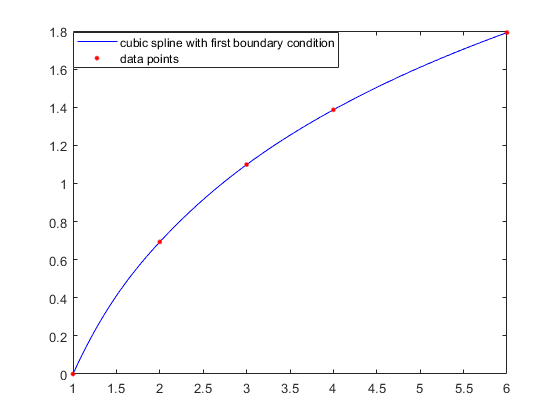
\includegraphics[width=0.8\textwidth]{cubic_log_first.png}
        \label{fig: cubic_log_first}
        \caption{一阶导数边界条件}
    \end{figure}
    \begin{figure}[H]
        \centering
        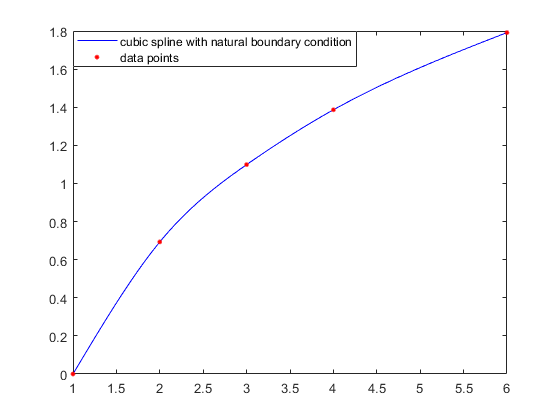
\includegraphics[width=0.8\textwidth]{cubic_log_natural.png}
        \label{fig: cubic_log_natural}
        \caption{自然边界条件}
    \end{figure}
    \begin{figure}[H]
        \centering
        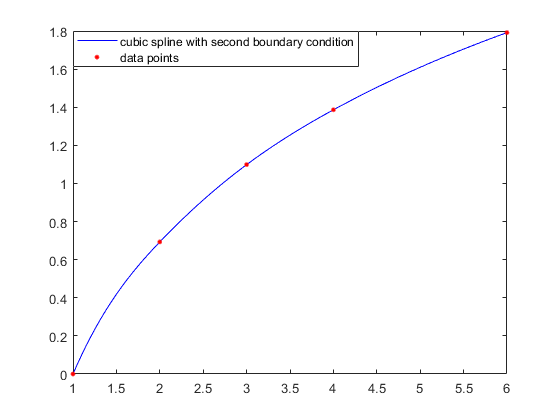
\includegraphics[width=0.8\textwidth]{cubic_log_second.png}
        \label{fig: cubic_log_second}
        \caption{二阶导数边界条件}
    \end{figure}
    \item 对区间$[-1,1]$进行均匀划分,分别令$N=6,11,21,41,81$为节点个数。使用一阶边界条件的三次样条函数在这些节点处进行插值,
    发现三次插值样条函数有效缓解了Runge现象。
    \begin{figure}[H]
        \centering
        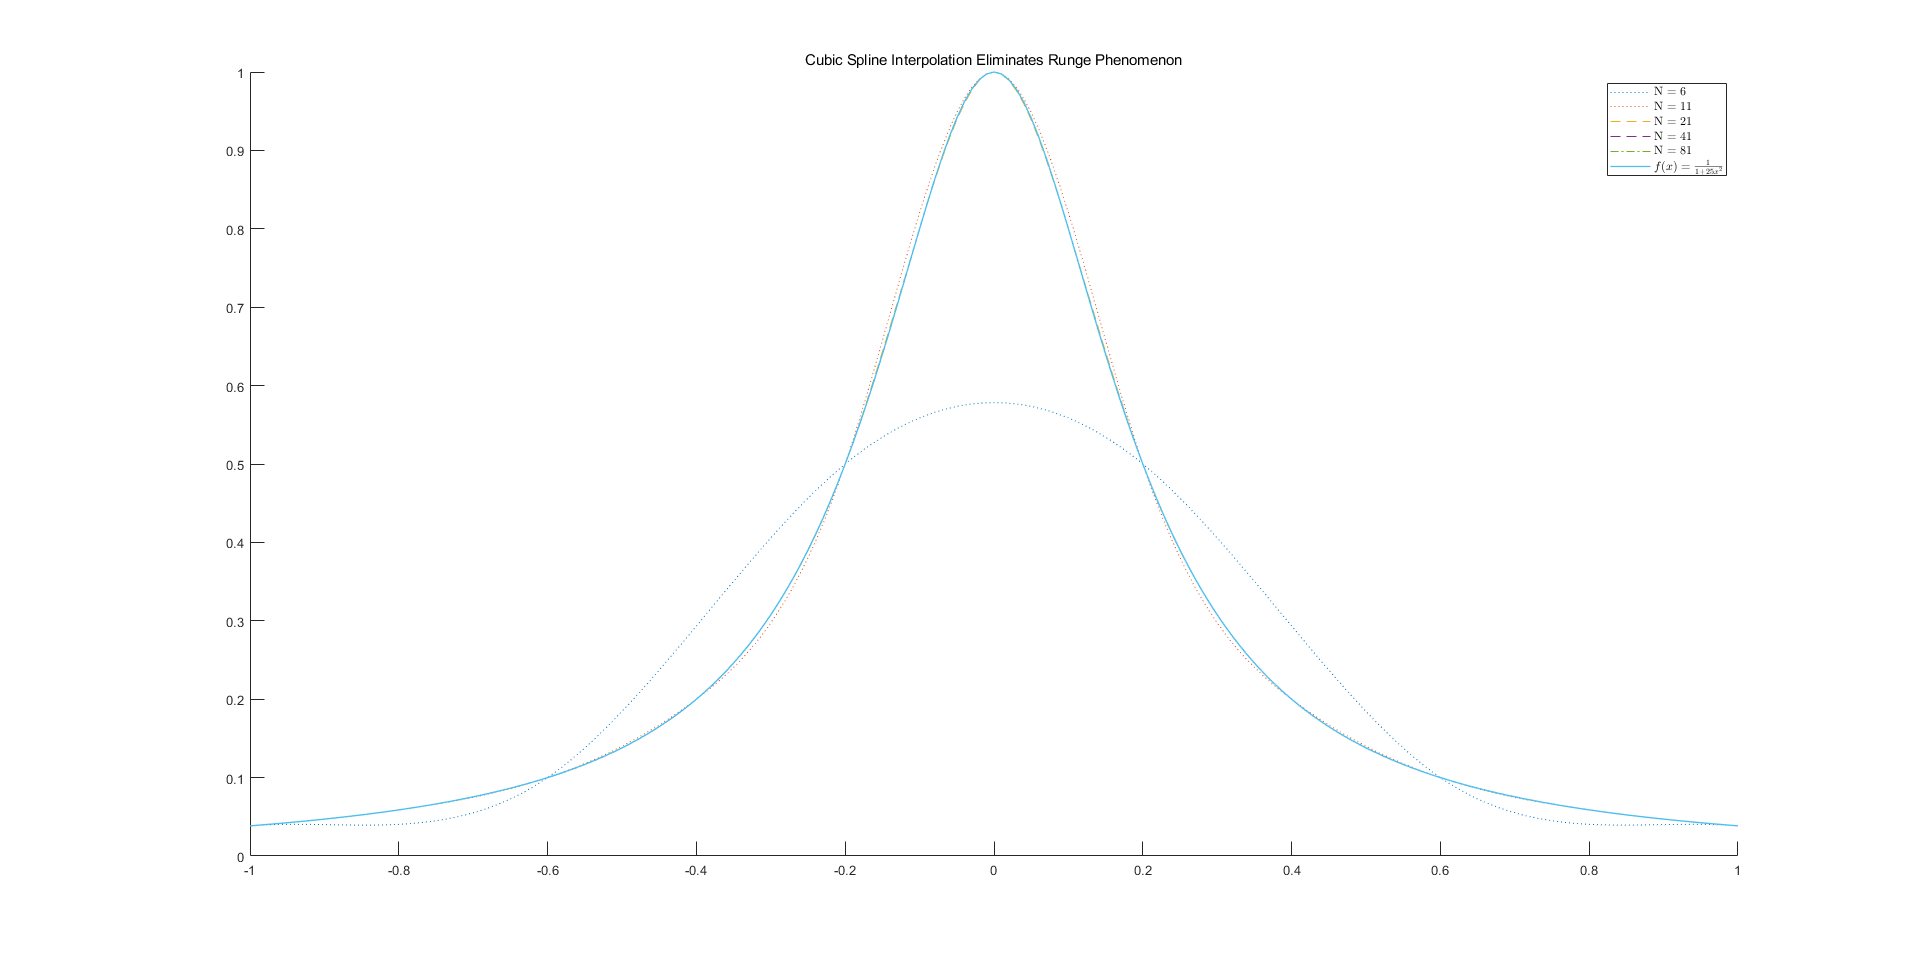
\includegraphics[width=1.0\textwidth]{runge_spline.png}
        \label{fig: runge_spline}
        \caption{三次插值样条函数有效缓解了Runge现象}
    \end{figure}
\end{itemize}

\section*{思考题 2}
\begin{enumerate}
    \item \textbf{引入半节点的原因}\\
    二次样条插值的基本目标是在每个分段区间内构造二次多项式,并通过设置合适的边界条件来保证插值函数的光滑性。通过引入半节点:
    \begin{itemize}
        \item 可以将每个分段的多项式划分得更加细致,增强插值函数的适应性;
        \item 保证插值函数在每个区间内具有良好的光滑性。
    \end{itemize}
    \item \textbf{不使用半节点,如何构造二次样条插值函数}\\
    如果仅使用原区间的分割点来构造二次样条插值函数,需要添加平滑性条件和边界条件:
    \begin{itemize}
        \item 为了保证插值函数的平滑性,需要保证样条函数在相邻区间的连接处具有连续的一阶导数;
        \item 添加自然边界条件或者固定斜率边界条件。
    \end{itemize}
\end{enumerate}

\end{document}
